The goal here is to computed the time evolution of the concurrence $C(\rho (t))$ in the lattice 
\refig{fig:Schematic of the lattice of the spin chain}
with the Hamiltonian of the XY and DMI.
For that with have two approch a numerical approch with the language of programmation Python and the 
analytical approch.

\subsection{Numerical approch}

To simulation the evolution of the concurrence \refdef{def: concurrence} we have to computed the 
density matrix but the necessery 
condition to computed the density matrix $\rho(t)$ in to found 
the state at the time $t$ the quantum system. For that 
we use the postulat of the evolution of the quantum system the Schrodïnger equation \cite{cohen-tannoudji_quantum_2019}. 

\begin{equation}\label{eq: Schrodïnger eq}
    \forall t \in \mathbb{R}_+, \ i \hbar \partial_t \ket{\psi(t)} = \hamil(t) \ket{\psi (t)} 
\end{equation}

Now let explain a generic algorithm to solve the Schrodïnger equation.

First let introduce the evolution operator $ \opevolution{t_0}$ which maps $ \ket{\psi(t_0)}$ the inital state of 
the system into $\ket{\psi(t)} $  

\begin{equation}\label{def : evolution operator}
   \forall t \in \mathbb{R}_+, \ \ketpsit = \opevolution{t_0}  \ket{\psi(t_0)} 
   \text{ with  } \ \opevolution{t_0} \opevolution{t_0}^\dagger = \opevolution{t_0}^\dagger \opevolution{t_0} = \text{id}  
\end{equation}

where $\text{id}$ is the identity function and $\opevolution{t_0}^\dagger$ is the adjoint of $\opevolution{t_0}$.
Now we start by considering a Hamiltonian \( \hamil(t) \) which is piecewise constant, i.e.,


\begin{equation}\label{prop: hypothese Hamiltionan}
    \forall j \in \mathbb{N}, \  \hamil(t) = \hamil(t_j) \quad \text{for} \quad t_j < t < t_{j+1},     
\end{equation}

where \( t_j \) are time steps at which the Hamiltonian changes suddenly.
\graphli{0.7}{methodology/constante_H.pdf}{Schematic of the \refprop{prop: hypothese Hamiltionan}}{hypothese Hamiltionan}

But now with the \refprop{prop: hypothese Hamiltionan}, the \refdef{def : evolution operator} and the \myeqref{eq: Schrodïnger eq}
we can express the $\opevolution{t_0}$ like this :

\begin{equation}
    \opevolution{t_0} = e^{-i \hamil (t-t_0)/\hbar}
\end{equation}



If we know the state of the quantum system at \( t_0 \), then we can compute the state quantum system at time \( t_n \) with $n > 0$ as:

\begin{align*}
    \ketpsitime{t_1} &= e^{-i \hamil (t_0) (t_1-t_0)/\hbar} \ketpsitime{t_0} \\
    \ketpsitime{t_2} &= e^{-i \hamil (t_1) (t_2-t_1)/\hbar} \ketpsitime{t_1} =  e^{-i \hamil(t_1) (t_2-t_1)/\hbar} 
    e^{-i \hamil(t_0) (t_1-t_0)/\hbar} \ketpsitime{t_0}\\
    &\vdots \\
    \ketpsitime{t_n} &= e^{-i \hamil(t_{n-1}) (t_n-t_{n-1})/\hbar} \ketpsitime{t_{n-1}} \cdots  e^{-i \hamil(t_{0}) (t_2-t_1)/\hbar} 
    e^{-i \hamil (t_1-t_0)/\hbar} \ketpsitime{t_0}
\end{align*}

Let us consider equally spaced time intervals:

\[
t_j = t_0 + j \Delta t.
\]

So the state of the quantum system at the time $t_n$ is  :
\begin{equation} \label{eq: expression state t_n}
   \forall n \in \mathbb{N}^*, \  \ketpsitime{t_n} = \prod_{i=0}^{n-1} e^{-i \hamil(t_{i}) \Delta t /\hbar} \ketpsitime{t_0}
\end{equation}

Notice the temporal order of operators \( \mathcal{U}(t_j, t_{j-1}) \) with \( t_j > t_{j-1} \). Operators later in time appear to the left.

So with deduce this algorithm to solve the Schrodïnger equation :
\begin{algorithm}[H]
    \caption{Solve Time-Dependent Schrödinger Equation}
    \begin{algorithmic}[1]
    \Procedure{solve}{$n: \text{integer}, t_f: \text{integer}, \text{Hamil: function}, \ketpsitime{t_0}: \text{array}$}
    \State $\Delta t \gets \frac{t_f}{n}$
    \State $\text{times} \gets \text{linspace}(0, t_f, n)$
    \State $\text{state\_t} \gets \text{empty list}$
    
    \For{$j = 0$ \textbf{to} $\text{length of times} - 1$}
        \State $\hamil(t_j) \gets \text{Hamil(times}[j])$
        \State $\mathcal{U}(t_{j+1}-t_j) \gets \text{matrix\_exponential}\left(-i \times \hamil(t_j) \times \Delta t \right)$
        \State $\ket{\psi(t_{j+1})} \gets \text{matrix\_dot\_product}(\mathcal{U}(t_{j+1}-t_j), \ket{\psi(t_0)})$
        \State \text{append } $\ket{\psi(t_{j+1})}$ \text{ to state\_t}
        \State $\ket{\psi(t_0)} \gets \ket{\psi(t_{j+1})}$
    \EndFor
    
    \State \Return $\text{state\_t}$
    \EndProcedure
    \end{algorithmic}
\end{algorithm}

\newpage 


Now we can compute the density matrix at the time $t$ but here if the length of the lattice is $L>1$ we can not 
compute the $C(\rho (t))$ according at the \refdef{def: concurrence} the concurrence in between only two qubits but if $L>1$ 
we have more of 2 qubits in the lattice so we can't use the  of the concurrence. 
Let see a example with 3 qubits to solve the problem in the figure :

\begin{figure}[h!]
    \centering
    \begin{subfigure}[b]{0.3\textwidth}
        \centering
        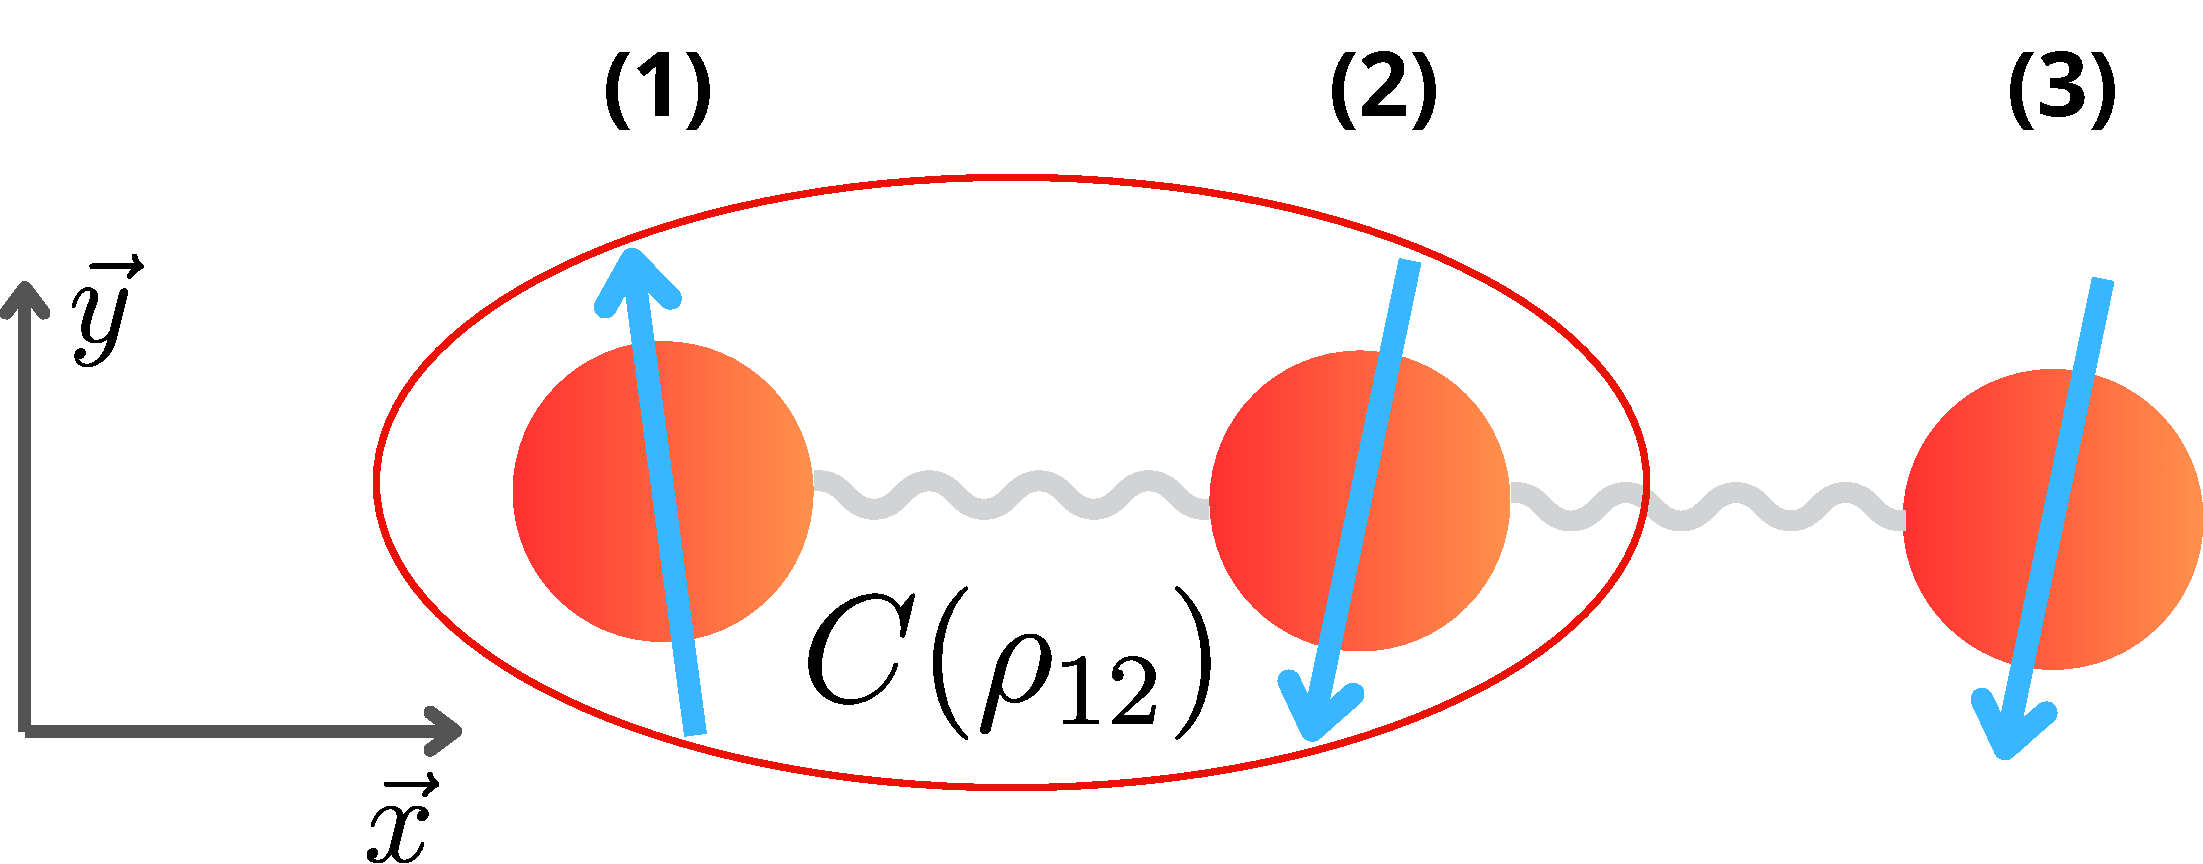
\includegraphics[width=\textwidth]{methodology/partial_trace_1.pdf}
        \caption{\centering Concurrence between the qubit (1) and (2)}
        \label{fig:Concurrence between the qubit (1) and (2)}
    \end{subfigure}
    \hfill
    \begin{subfigure}[b]{0.3\textwidth}
        \centering
        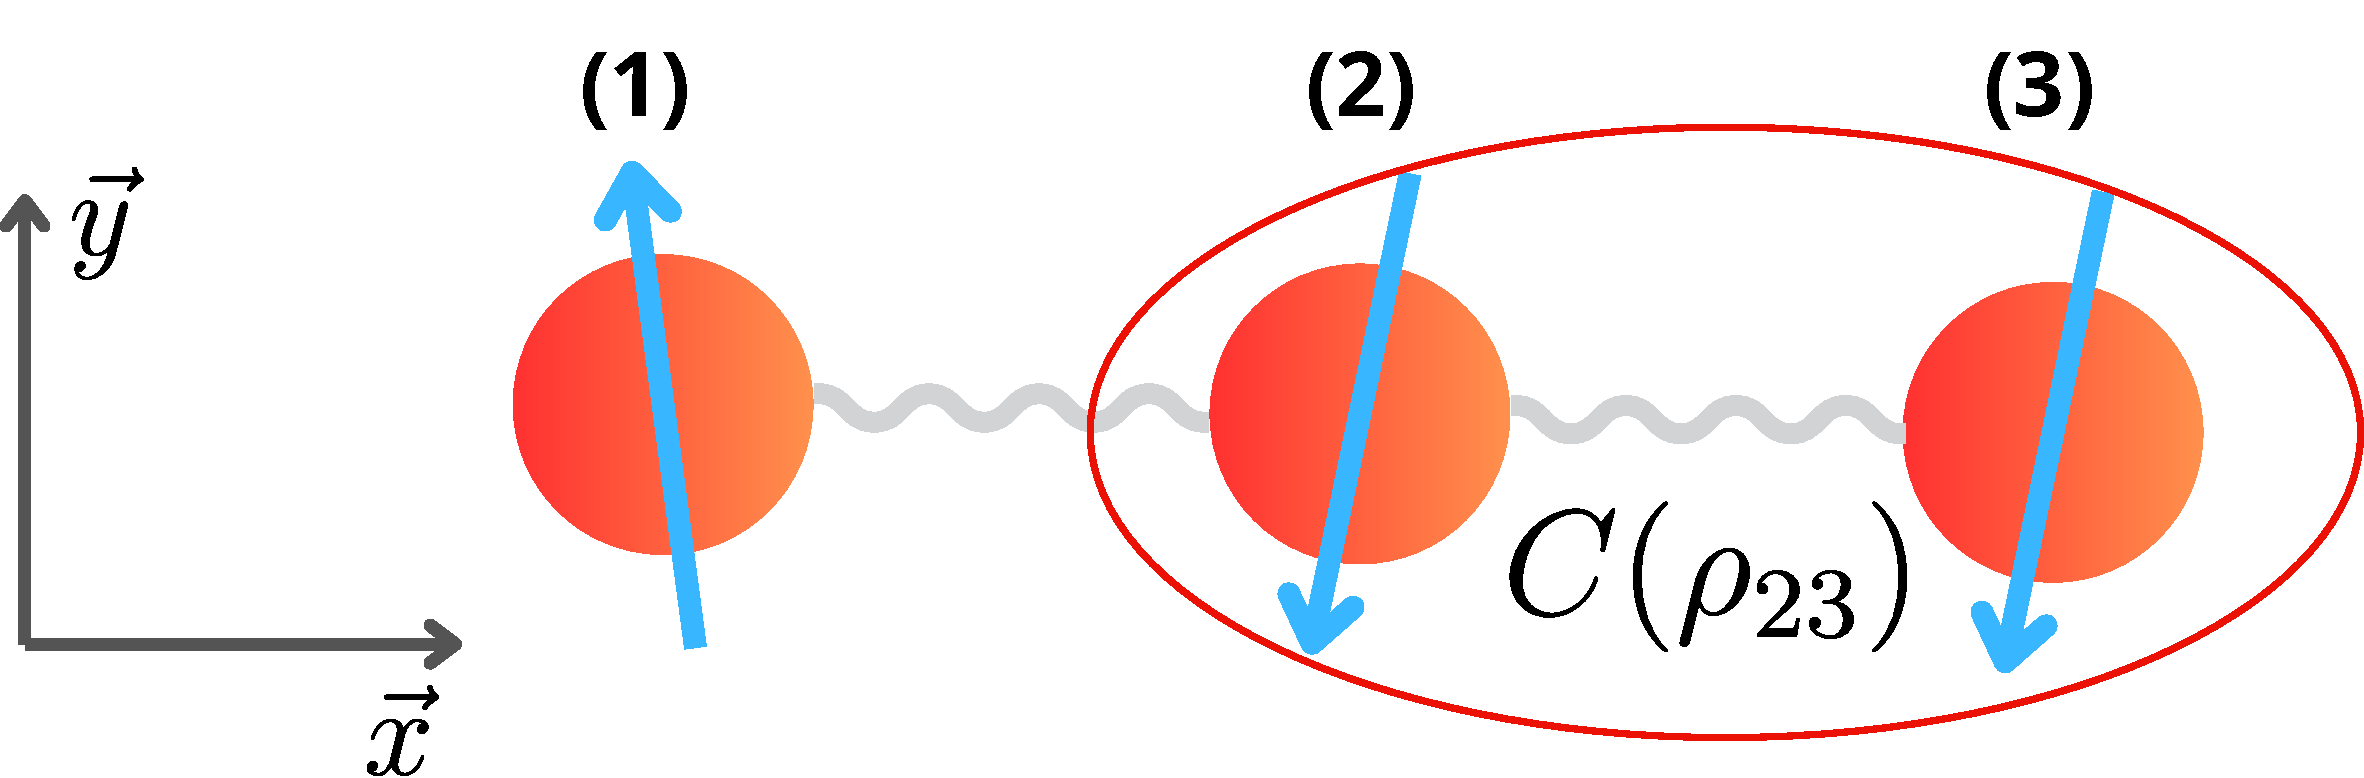
\includegraphics[width=\textwidth]{methodology/partial_trace_2.pdf}
        \caption{\centering Concurrence between the qubit (2) and (3)}
        \label{fig:Concurrence between the qubit (2) and (3)}
    \end{subfigure}
    \hfill
    \begin{subfigure}[b]{0.3\textwidth}
        \centering
        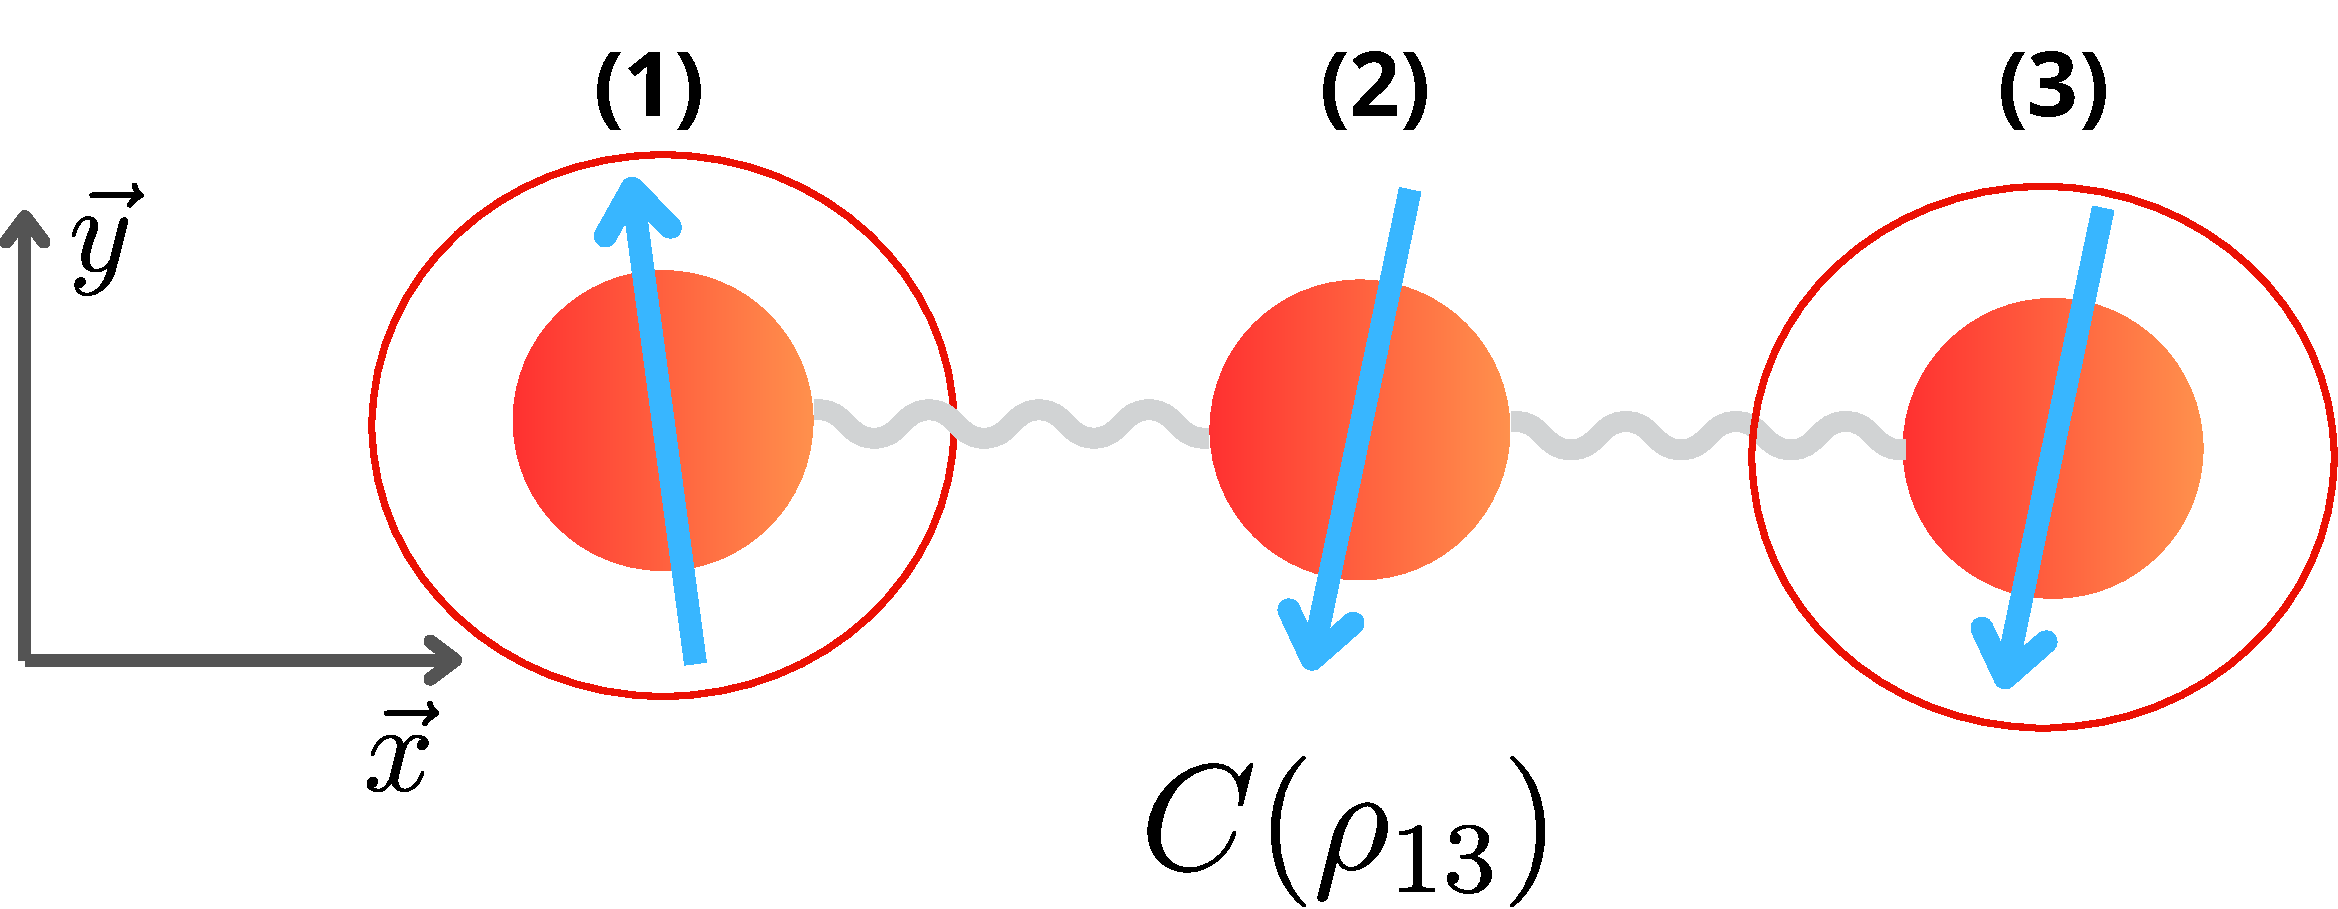
\includegraphics[width=\textwidth]{methodology/partial_trace_3.pdf}
        \caption{\centering Concurrence between the qubit (1) and (3)}
        \label{fig:Concurrence between the qubit (1) and (3)}
    \end{subfigure}
    \caption{Problem of calculation of the concurrence for many qubits}
    \label{fig:partial_traces}
\end{figure}



We understand we the \refig{fig:partial_traces} with have to a isolate the pair of the qubit and computed the density matrix of the 
couple of qubit note $\rho_{ij}$ where $i \neq j \text{ and } (i,j) \in \mathbb{N}^*$, for that we will use a mathematical tool call the partial
trace \cite{bradley_at_2020} 

\mydef{Partial trace}{
Let take a system of $L+1$ quantum system so 

\begin{equation}
    (i,j) \in (\mathbb{N}^*)^2 \text{ and } i \neq j , \ \rho_{ij} = \sumd{i=1}{\dim(A)} \bra*{e_i} \rho \ket{e_i}
\end{equation}

}{}

Let do a example
For example if we want to compute the density matrix of the system of the qubit (1) and (2) schematic 
in the \refig{fig:Concurrence between the qubit (1) and (2)} 




